% Copyright © 2013 Martin Ueding <dev@martin-ueding.de>

% Copyright © 2012-2013 Martin Ueding <dev@martin-ueding.de>

% This is my general purpose LaTeX header file for writing German documents.
% Ideally, you include this using a simple ``% Copyright © 2012-2013 Martin Ueding <dev@martin-ueding.de>

% This is my general purpose LaTeX header file for writing German documents.
% Ideally, you include this using a simple ``% Copyright © 2012-2013 Martin Ueding <dev@martin-ueding.de>

% This is my general purpose LaTeX header file for writing German documents.
% Ideally, you include this using a simple ``\input{header.tex}`` in your main
% document and start with ``\title`` and ``\begin{document}`` afterwards.

% If you need to add additional packages, I recommend not doing this in this
% file, but in your main document. That way, you can just drop in a new
% ``header.tex`` and get all the new commands without having to merge manually.

% Since this file encorporates a CC-BY-SA fragment, this whole files is
% licensed under the CC-BY-SA license.

\documentclass[11pt, ngerman, fleqn, DIV=15, BCOR=2cm, headinclude]{scrartcl}

\usepackage{graphicx}

% Environment to quote the problem. Currently, this is just a new name for the
% quote environment.
\newenvironment{problem}{\begin{quote}\textsf{\textbf{Aufgabenstellung:}}\quad}{\end{quote}}

\setkomafont{caption}{\sf}
\setkomafont{captionlabel}{\usekomafont{caption}}

%%%%%%%%%%%%%%%%%%%%%%%%%%%%%%%%%%%%%%%%%%%%%%%%%%%%%%%%%%%%%%%%%%%%%%%%%%%%%%%
%                                Locale, date                                 %
%%%%%%%%%%%%%%%%%%%%%%%%%%%%%%%%%%%%%%%%%%%%%%%%%%%%%%%%%%%%%%%%%%%%%%%%%%%%%%%

\usepackage{babel}
\usepackage[iso]{isodate}

%%%%%%%%%%%%%%%%%%%%%%%%%%%%%%%%%%%%%%%%%%%%%%%%%%%%%%%%%%%%%%%%%%%%%%%%%%%%%%%
%                          Margins and other spacing                          %
%%%%%%%%%%%%%%%%%%%%%%%%%%%%%%%%%%%%%%%%%%%%%%%%%%%%%%%%%%%%%%%%%%%%%%%%%%%%%%%

\usepackage[parfill]{parskip}
\usepackage{setspace}
\usepackage[activate]{microtype}

\setlength{\columnsep}{2cm}

%%%%%%%%%%%%%%%%%%%%%%%%%%%%%%%%%%%%%%%%%%%%%%%%%%%%%%%%%%%%%%%%%%%%%%%%%%%%%%%
%                                    Color                                    %
%%%%%%%%%%%%%%%%%%%%%%%%%%%%%%%%%%%%%%%%%%%%%%%%%%%%%%%%%%%%%%%%%%%%%%%%%%%%%%%

\usepackage[usenames, dvipsnames]{xcolor}

\colorlet{darkred}{red!70!black}
\colorlet{darkblue}{blue!70!black}
\colorlet{darkgreen}{green!40!black}

%%%%%%%%%%%%%%%%%%%%%%%%%%%%%%%%%%%%%%%%%%%%%%%%%%%%%%%%%%%%%%%%%%%%%%%%%%%%%%%
%                         Font and font like settings                         %
%%%%%%%%%%%%%%%%%%%%%%%%%%%%%%%%%%%%%%%%%%%%%%%%%%%%%%%%%%%%%%%%%%%%%%%%%%%%%%%

% This replaces all fonts with Bitstream Charter, Bitstream Vera Sans and
% Bitstream Vera Mono. Math will be rendered in Charter.
\usepackage[charter, greekuppercase=italicized]{mathdesign}
\usepackage{beramono}
\usepackage{berasans}

% Bold, sans-serif tensors. This fragment is taken from “egreg” from
% http://tex.stackexchange.com/a/82747/8945 and licensed under `CC-BY-SA
% <https://creativecommons.org/licenses/by-sa/3.0/>`_.
\usepackage{bm}
\DeclareMathAlphabet{\mathsfit}{\encodingdefault}{\sfdefault}{m}{sl}
\SetMathAlphabet{\mathsfit}{bold}{\encodingdefault}{\sfdefault}{bx}{sl}
\newcommand{\tens}[1]{\bm{\mathsfit{#1}}}

% Bold vectors.
\renewcommand{\vec}[1]{\boldsymbol{#1}}

%%%%%%%%%%%%%%%%%%%%%%%%%%%%%%%%%%%%%%%%%%%%%%%%%%%%%%%%%%%%%%%%%%%%%%%%%%%%%%%
%                               Input encoding                                %
%%%%%%%%%%%%%%%%%%%%%%%%%%%%%%%%%%%%%%%%%%%%%%%%%%%%%%%%%%%%%%%%%%%%%%%%%%%%%%%

\usepackage[T1]{fontenc}
\usepackage[utf8]{inputenc}

%%%%%%%%%%%%%%%%%%%%%%%%%%%%%%%%%%%%%%%%%%%%%%%%%%%%%%%%%%%%%%%%%%%%%%%%%%%%%%%
%                         Hyperrefs and PDF metadata                          %
%%%%%%%%%%%%%%%%%%%%%%%%%%%%%%%%%%%%%%%%%%%%%%%%%%%%%%%%%%%%%%%%%%%%%%%%%%%%%%%

\usepackage{hyperref}
\usepackage{lastpage}

% This sets the author in the properties of the PDF as well. If you want to
% change it, just override it with another ``\hypersetup`` call.
\hypersetup{
	breaklinks=false,
	citecolor=darkgreen,
	colorlinks=true,
	linkcolor=darkblue,
	menucolor=black,
	pdfauthor={Martin Ueding},
	urlcolor=darkblue,
}

%%%%%%%%%%%%%%%%%%%%%%%%%%%%%%%%%%%%%%%%%%%%%%%%%%%%%%%%%%%%%%%%%%%%%%%%%%%%%%%
%                               Math Operators                                %
%%%%%%%%%%%%%%%%%%%%%%%%%%%%%%%%%%%%%%%%%%%%%%%%%%%%%%%%%%%%%%%%%%%%%%%%%%%%%%%

% AMS environments like ``align`` and theorems like ``proof``.
\usepackage{amsmath}
\usepackage{amsthm}

% Common math constructs like partial derivatives.
\usepackage{commath}

% Physical units.
\usepackage[output-decimal-marker={,}]{siunitx}

% Since I use mathdesign with italic uppercase greek characters, the Ohm unit will be displayed with an italic Ω by default. Units have to be roman, so this forces it the right way.
\DeclareSIUnit{\ohm}{$\Omegaup$}
\DeclareSIUnit{\division}{DIV}
\DeclareSIUnit{\voltss}{$\mathrm{V_{SS}}$}

% Word like operators.
\DeclareMathOperator{\acosh}{arcosh}
\DeclareMathOperator{\arcosh}{arcosh}
\DeclareMathOperator{\arcsinh}{arsinh}
\DeclareMathOperator{\arsinh}{arsinh}
\DeclareMathOperator{\asinh}{arsinh}
\DeclareMathOperator{\card}{card}
\DeclareMathOperator{\csch}{cshs}
\DeclareMathOperator{\diam}{diam}
\DeclareMathOperator{\sech}{sech}
\renewcommand{\Im}{\mathop{{}\mathrm{Im}}\nolimits}
\renewcommand{\Re}{\mathop{{}\mathrm{Re}}\nolimits}

% Fourier transform.
\DeclareMathOperator{\fourier}{\ensuremath{\mathcal{F}}}

% Roman versions of “e” and “i” to serve as Euler's number and the imaginary
% constant.
\newcommand{\ee}{\eup}
\newcommand{\eup}{\mathrm e}
\newcommand{\ii}{\iup}
\newcommand{\iup}{\mathrm i}

% Symbols for the various mathematical fields (natural numbers, integers,
% rational numbers, real numbers, complex numbers).
\newcommand{\C}{\ensuremath{\mathbb C}}
\newcommand{\N}{\ensuremath{\mathbb N}}
\newcommand{\Q}{\ensuremath{\mathbb Q}}
\newcommand{\R}{\ensuremath{\mathbb R}}
\newcommand{\Z}{\ensuremath{\mathbb Z}}

% Shape like operators.
\DeclareMathOperator{\dalambert}{\Box}
\DeclareMathOperator{\laplace}{\bigtriangleup}
\newcommand{\curl}{\vnabla \times}
\newcommand{\divergence}[1]{\inner{\vnabla}{#1}}
\newcommand{\vnabla}{\vec \nabla}

\newcommand{\half}{\frac 12}

% Unit vector (German „Einheitsvektor“).
\newcommand{\ev}{\hat{\vec e}}

% Scientific notation for large numbers.
\newcommand{\e}[1]{\cdot 10^{#1}}

% Mathematician's notation for the inner (scalar, dot) product.
\newcommand{\bracket}[1]{\left\langle #1 \right\rangle}
\newcommand{\inner}[2]{\bracket{#1, #2}}

% Placeholders.
\newcommand{\emesswert}{\del{\messwert \pm \messwert}}
\newcommand{\fehlt}{\textcolor{darkred}{Hier fehlen noch Inhalte.}}
\newcommand{\messwert}{\textcolor{blue}{\square}}
\newcommand{\punkte}{\phantom{xxxxx}}
\newcommand{\punktevon}[1]{\begin{flushright}/ #1\end{flushright}}

% Separator for equations on a single line.
\newcommand{\eqnsep}{,\quad}

% Quantum Mechanics
\usepackage{braket}

%%%%%%%%%%%%%%%%%%%%%%%%%%%%%%%%%%%%%%%%%%%%%%%%%%%%%%%%%%%%%%%%%%%%%%%%%%%%%%%
%                                  Headings                                   %
%%%%%%%%%%%%%%%%%%%%%%%%%%%%%%%%%%%%%%%%%%%%%%%%%%%%%%%%%%%%%%%%%%%%%%%%%%%%%%%

% This will set fancy headings to the top of the page. The page number will be
% accompanied by the total number of pages. That way, you will know if any page
% is missing.
%
% If you do not want this for your document, you can just use
% ``\pagestyle{plain}``.

\usepackage{scrpage2}

\pagestyle{scrheadings}
\automark{section}
\cfoot{\footnotesize{Seite \thepage\ / \pageref{LastPage}}}
\chead{}
\ihead{}
\ohead{\rightmark}
\setheadsepline{.4pt}

%%%%%%%%%%%%%%%%%%%%%%%%%%%%%%%%%%%%%%%%%%%%%%%%%%%%%%%%%%%%%%%%%%%%%%%%%%%%%%%
%                            Bibliography (BibTeX)                            %
%%%%%%%%%%%%%%%%%%%%%%%%%%%%%%%%%%%%%%%%%%%%%%%%%%%%%%%%%%%%%%%%%%%%%%%%%%%%%%%

\newcommand{\bibliographyfile}{../../central-bibtex/Central}
\bibliographystyle{apalike2}

%%%%%%%%%%%%%%%%%%%%%%%%%%%%%%%%%%%%%%%%%%%%%%%%%%%%%%%%%%%%%%%%%%%%%%%%%%%%%%%
%                                Abbreviations                                %
%%%%%%%%%%%%%%%%%%%%%%%%%%%%%%%%%%%%%%%%%%%%%%%%%%%%%%%%%%%%%%%%%%%%%%%%%%%%%%%

\newcommand{\dhabk}{\mbox{d.\,h.}}

%%%%%%%%%%%%%%%%%%%%%%%%%%%%%%%%%%%%%%%%%%%%%%%%%%%%%%%%%%%%%%%%%%%%%%%%%%%%%%%
%                                  Licences                                   %
%%%%%%%%%%%%%%%%%%%%%%%%%%%%%%%%%%%%%%%%%%%%%%%%%%%%%%%%%%%%%%%%%%%%%%%%%%%%%%%

\usepackage{ccicons}

\newcommand{\ccbysadetext}{%
	\begin{small}
		Dieses Werk bzw. Inhalt steht unter einer
		\href{http://creativecommons.org/licenses/by-sa/3.0/deed.de}{%
			Creative Commons Namensnennung - Weitergabe unter gleichen
		Bedingungen 3.0 Unported Lizenz}.
	\end{small}
}

\newcommand{\ccbysadetitle}{%
	Lizenz: \href{http://creativecommons.org/licenses/by-sa/3.0/deed.de}
	{CC-BY-SA 3.0 \ccbysa}
}
`` in your main
% document and start with ``\title`` and ``\begin{document}`` afterwards.

% If you need to add additional packages, I recommend not doing this in this
% file, but in your main document. That way, you can just drop in a new
% ``header.tex`` and get all the new commands without having to merge manually.

% Since this file encorporates a CC-BY-SA fragment, this whole files is
% licensed under the CC-BY-SA license.

\documentclass[11pt, ngerman, fleqn, DIV=15, BCOR=2cm, headinclude]{scrartcl}

\usepackage{graphicx}

% Environment to quote the problem. Currently, this is just a new name for the
% quote environment.
\newenvironment{problem}{\begin{quote}\textsf{\textbf{Aufgabenstellung:}}\quad}{\end{quote}}

\setkomafont{caption}{\sf}
\setkomafont{captionlabel}{\usekomafont{caption}}

%%%%%%%%%%%%%%%%%%%%%%%%%%%%%%%%%%%%%%%%%%%%%%%%%%%%%%%%%%%%%%%%%%%%%%%%%%%%%%%
%                                Locale, date                                 %
%%%%%%%%%%%%%%%%%%%%%%%%%%%%%%%%%%%%%%%%%%%%%%%%%%%%%%%%%%%%%%%%%%%%%%%%%%%%%%%

\usepackage{babel}
\usepackage[iso]{isodate}

%%%%%%%%%%%%%%%%%%%%%%%%%%%%%%%%%%%%%%%%%%%%%%%%%%%%%%%%%%%%%%%%%%%%%%%%%%%%%%%
%                          Margins and other spacing                          %
%%%%%%%%%%%%%%%%%%%%%%%%%%%%%%%%%%%%%%%%%%%%%%%%%%%%%%%%%%%%%%%%%%%%%%%%%%%%%%%

\usepackage[parfill]{parskip}
\usepackage{setspace}
\usepackage[activate]{microtype}

\setlength{\columnsep}{2cm}

%%%%%%%%%%%%%%%%%%%%%%%%%%%%%%%%%%%%%%%%%%%%%%%%%%%%%%%%%%%%%%%%%%%%%%%%%%%%%%%
%                                    Color                                    %
%%%%%%%%%%%%%%%%%%%%%%%%%%%%%%%%%%%%%%%%%%%%%%%%%%%%%%%%%%%%%%%%%%%%%%%%%%%%%%%

\usepackage[usenames, dvipsnames]{xcolor}

\colorlet{darkred}{red!70!black}
\colorlet{darkblue}{blue!70!black}
\colorlet{darkgreen}{green!40!black}

%%%%%%%%%%%%%%%%%%%%%%%%%%%%%%%%%%%%%%%%%%%%%%%%%%%%%%%%%%%%%%%%%%%%%%%%%%%%%%%
%                         Font and font like settings                         %
%%%%%%%%%%%%%%%%%%%%%%%%%%%%%%%%%%%%%%%%%%%%%%%%%%%%%%%%%%%%%%%%%%%%%%%%%%%%%%%

% This replaces all fonts with Bitstream Charter, Bitstream Vera Sans and
% Bitstream Vera Mono. Math will be rendered in Charter.
\usepackage[charter, greekuppercase=italicized]{mathdesign}
\usepackage{beramono}
\usepackage{berasans}

% Bold, sans-serif tensors. This fragment is taken from “egreg” from
% http://tex.stackexchange.com/a/82747/8945 and licensed under `CC-BY-SA
% <https://creativecommons.org/licenses/by-sa/3.0/>`_.
\usepackage{bm}
\DeclareMathAlphabet{\mathsfit}{\encodingdefault}{\sfdefault}{m}{sl}
\SetMathAlphabet{\mathsfit}{bold}{\encodingdefault}{\sfdefault}{bx}{sl}
\newcommand{\tens}[1]{\bm{\mathsfit{#1}}}

% Bold vectors.
\renewcommand{\vec}[1]{\boldsymbol{#1}}

%%%%%%%%%%%%%%%%%%%%%%%%%%%%%%%%%%%%%%%%%%%%%%%%%%%%%%%%%%%%%%%%%%%%%%%%%%%%%%%
%                               Input encoding                                %
%%%%%%%%%%%%%%%%%%%%%%%%%%%%%%%%%%%%%%%%%%%%%%%%%%%%%%%%%%%%%%%%%%%%%%%%%%%%%%%

\usepackage[T1]{fontenc}
\usepackage[utf8]{inputenc}

%%%%%%%%%%%%%%%%%%%%%%%%%%%%%%%%%%%%%%%%%%%%%%%%%%%%%%%%%%%%%%%%%%%%%%%%%%%%%%%
%                         Hyperrefs and PDF metadata                          %
%%%%%%%%%%%%%%%%%%%%%%%%%%%%%%%%%%%%%%%%%%%%%%%%%%%%%%%%%%%%%%%%%%%%%%%%%%%%%%%

\usepackage{hyperref}
\usepackage{lastpage}

% This sets the author in the properties of the PDF as well. If you want to
% change it, just override it with another ``\hypersetup`` call.
\hypersetup{
	breaklinks=false,
	citecolor=darkgreen,
	colorlinks=true,
	linkcolor=darkblue,
	menucolor=black,
	pdfauthor={Martin Ueding},
	urlcolor=darkblue,
}

%%%%%%%%%%%%%%%%%%%%%%%%%%%%%%%%%%%%%%%%%%%%%%%%%%%%%%%%%%%%%%%%%%%%%%%%%%%%%%%
%                               Math Operators                                %
%%%%%%%%%%%%%%%%%%%%%%%%%%%%%%%%%%%%%%%%%%%%%%%%%%%%%%%%%%%%%%%%%%%%%%%%%%%%%%%

% AMS environments like ``align`` and theorems like ``proof``.
\usepackage{amsmath}
\usepackage{amsthm}

% Common math constructs like partial derivatives.
\usepackage{commath}

% Physical units.
\usepackage[output-decimal-marker={,}]{siunitx}

% Since I use mathdesign with italic uppercase greek characters, the Ohm unit will be displayed with an italic Ω by default. Units have to be roman, so this forces it the right way.
\DeclareSIUnit{\ohm}{$\Omegaup$}
\DeclareSIUnit{\division}{DIV}
\DeclareSIUnit{\voltss}{$\mathrm{V_{SS}}$}

% Word like operators.
\DeclareMathOperator{\acosh}{arcosh}
\DeclareMathOperator{\arcosh}{arcosh}
\DeclareMathOperator{\arcsinh}{arsinh}
\DeclareMathOperator{\arsinh}{arsinh}
\DeclareMathOperator{\asinh}{arsinh}
\DeclareMathOperator{\card}{card}
\DeclareMathOperator{\csch}{cshs}
\DeclareMathOperator{\diam}{diam}
\DeclareMathOperator{\sech}{sech}
\renewcommand{\Im}{\mathop{{}\mathrm{Im}}\nolimits}
\renewcommand{\Re}{\mathop{{}\mathrm{Re}}\nolimits}

% Fourier transform.
\DeclareMathOperator{\fourier}{\ensuremath{\mathcal{F}}}

% Roman versions of “e” and “i” to serve as Euler's number and the imaginary
% constant.
\newcommand{\ee}{\eup}
\newcommand{\eup}{\mathrm e}
\newcommand{\ii}{\iup}
\newcommand{\iup}{\mathrm i}

% Symbols for the various mathematical fields (natural numbers, integers,
% rational numbers, real numbers, complex numbers).
\newcommand{\C}{\ensuremath{\mathbb C}}
\newcommand{\N}{\ensuremath{\mathbb N}}
\newcommand{\Q}{\ensuremath{\mathbb Q}}
\newcommand{\R}{\ensuremath{\mathbb R}}
\newcommand{\Z}{\ensuremath{\mathbb Z}}

% Shape like operators.
\DeclareMathOperator{\dalambert}{\Box}
\DeclareMathOperator{\laplace}{\bigtriangleup}
\newcommand{\curl}{\vnabla \times}
\newcommand{\divergence}[1]{\inner{\vnabla}{#1}}
\newcommand{\vnabla}{\vec \nabla}

\newcommand{\half}{\frac 12}

% Unit vector (German „Einheitsvektor“).
\newcommand{\ev}{\hat{\vec e}}

% Scientific notation for large numbers.
\newcommand{\e}[1]{\cdot 10^{#1}}

% Mathematician's notation for the inner (scalar, dot) product.
\newcommand{\bracket}[1]{\left\langle #1 \right\rangle}
\newcommand{\inner}[2]{\bracket{#1, #2}}

% Placeholders.
\newcommand{\emesswert}{\del{\messwert \pm \messwert}}
\newcommand{\fehlt}{\textcolor{darkred}{Hier fehlen noch Inhalte.}}
\newcommand{\messwert}{\textcolor{blue}{\square}}
\newcommand{\punkte}{\phantom{xxxxx}}
\newcommand{\punktevon}[1]{\begin{flushright}/ #1\end{flushright}}

% Separator for equations on a single line.
\newcommand{\eqnsep}{,\quad}

% Quantum Mechanics
\usepackage{braket}

%%%%%%%%%%%%%%%%%%%%%%%%%%%%%%%%%%%%%%%%%%%%%%%%%%%%%%%%%%%%%%%%%%%%%%%%%%%%%%%
%                                  Headings                                   %
%%%%%%%%%%%%%%%%%%%%%%%%%%%%%%%%%%%%%%%%%%%%%%%%%%%%%%%%%%%%%%%%%%%%%%%%%%%%%%%

% This will set fancy headings to the top of the page. The page number will be
% accompanied by the total number of pages. That way, you will know if any page
% is missing.
%
% If you do not want this for your document, you can just use
% ``\pagestyle{plain}``.

\usepackage{scrpage2}

\pagestyle{scrheadings}
\automark{section}
\cfoot{\footnotesize{Seite \thepage\ / \pageref{LastPage}}}
\chead{}
\ihead{}
\ohead{\rightmark}
\setheadsepline{.4pt}

%%%%%%%%%%%%%%%%%%%%%%%%%%%%%%%%%%%%%%%%%%%%%%%%%%%%%%%%%%%%%%%%%%%%%%%%%%%%%%%
%                            Bibliography (BibTeX)                            %
%%%%%%%%%%%%%%%%%%%%%%%%%%%%%%%%%%%%%%%%%%%%%%%%%%%%%%%%%%%%%%%%%%%%%%%%%%%%%%%

\newcommand{\bibliographyfile}{../../central-bibtex/Central}
\bibliographystyle{apalike2}

%%%%%%%%%%%%%%%%%%%%%%%%%%%%%%%%%%%%%%%%%%%%%%%%%%%%%%%%%%%%%%%%%%%%%%%%%%%%%%%
%                                Abbreviations                                %
%%%%%%%%%%%%%%%%%%%%%%%%%%%%%%%%%%%%%%%%%%%%%%%%%%%%%%%%%%%%%%%%%%%%%%%%%%%%%%%

\newcommand{\dhabk}{\mbox{d.\,h.}}

%%%%%%%%%%%%%%%%%%%%%%%%%%%%%%%%%%%%%%%%%%%%%%%%%%%%%%%%%%%%%%%%%%%%%%%%%%%%%%%
%                                  Licences                                   %
%%%%%%%%%%%%%%%%%%%%%%%%%%%%%%%%%%%%%%%%%%%%%%%%%%%%%%%%%%%%%%%%%%%%%%%%%%%%%%%

\usepackage{ccicons}

\newcommand{\ccbysadetext}{%
	\begin{small}
		Dieses Werk bzw. Inhalt steht unter einer
		\href{http://creativecommons.org/licenses/by-sa/3.0/deed.de}{%
			Creative Commons Namensnennung - Weitergabe unter gleichen
		Bedingungen 3.0 Unported Lizenz}.
	\end{small}
}

\newcommand{\ccbysadetitle}{%
	Lizenz: \href{http://creativecommons.org/licenses/by-sa/3.0/deed.de}
	{CC-BY-SA 3.0 \ccbysa}
}
`` in your main
% document and start with ``\title`` and ``\begin{document}`` afterwards.

% If you need to add additional packages, I recommend not doing this in this
% file, but in your main document. That way, you can just drop in a new
% ``header.tex`` and get all the new commands without having to merge manually.

% Since this file encorporates a CC-BY-SA fragment, this whole files is
% licensed under the CC-BY-SA license.

\documentclass[11pt, ngerman, fleqn, DIV=15, BCOR=2cm, headinclude]{scrartcl}

\usepackage{graphicx}

% Environment to quote the problem. Currently, this is just a new name for the
% quote environment.
\newenvironment{problem}{\begin{quote}\textsf{\textbf{Aufgabenstellung:}}\quad}{\end{quote}}

\setkomafont{caption}{\sf}
\setkomafont{captionlabel}{\usekomafont{caption}}

%%%%%%%%%%%%%%%%%%%%%%%%%%%%%%%%%%%%%%%%%%%%%%%%%%%%%%%%%%%%%%%%%%%%%%%%%%%%%%%
%                                Locale, date                                 %
%%%%%%%%%%%%%%%%%%%%%%%%%%%%%%%%%%%%%%%%%%%%%%%%%%%%%%%%%%%%%%%%%%%%%%%%%%%%%%%

\usepackage{babel}
\usepackage[iso]{isodate}

%%%%%%%%%%%%%%%%%%%%%%%%%%%%%%%%%%%%%%%%%%%%%%%%%%%%%%%%%%%%%%%%%%%%%%%%%%%%%%%
%                          Margins and other spacing                          %
%%%%%%%%%%%%%%%%%%%%%%%%%%%%%%%%%%%%%%%%%%%%%%%%%%%%%%%%%%%%%%%%%%%%%%%%%%%%%%%

\usepackage[parfill]{parskip}
\usepackage{setspace}
\usepackage[activate]{microtype}

\setlength{\columnsep}{2cm}

%%%%%%%%%%%%%%%%%%%%%%%%%%%%%%%%%%%%%%%%%%%%%%%%%%%%%%%%%%%%%%%%%%%%%%%%%%%%%%%
%                                    Color                                    %
%%%%%%%%%%%%%%%%%%%%%%%%%%%%%%%%%%%%%%%%%%%%%%%%%%%%%%%%%%%%%%%%%%%%%%%%%%%%%%%

\usepackage[usenames, dvipsnames]{xcolor}

\colorlet{darkred}{red!70!black}
\colorlet{darkblue}{blue!70!black}
\colorlet{darkgreen}{green!40!black}

%%%%%%%%%%%%%%%%%%%%%%%%%%%%%%%%%%%%%%%%%%%%%%%%%%%%%%%%%%%%%%%%%%%%%%%%%%%%%%%
%                         Font and font like settings                         %
%%%%%%%%%%%%%%%%%%%%%%%%%%%%%%%%%%%%%%%%%%%%%%%%%%%%%%%%%%%%%%%%%%%%%%%%%%%%%%%

% This replaces all fonts with Bitstream Charter, Bitstream Vera Sans and
% Bitstream Vera Mono. Math will be rendered in Charter.
\usepackage[charter, greekuppercase=italicized]{mathdesign}
\usepackage{beramono}
\usepackage{berasans}

% Bold, sans-serif tensors. This fragment is taken from “egreg” from
% http://tex.stackexchange.com/a/82747/8945 and licensed under `CC-BY-SA
% <https://creativecommons.org/licenses/by-sa/3.0/>`_.
\usepackage{bm}
\DeclareMathAlphabet{\mathsfit}{\encodingdefault}{\sfdefault}{m}{sl}
\SetMathAlphabet{\mathsfit}{bold}{\encodingdefault}{\sfdefault}{bx}{sl}
\newcommand{\tens}[1]{\bm{\mathsfit{#1}}}

% Bold vectors.
\renewcommand{\vec}[1]{\boldsymbol{#1}}

%%%%%%%%%%%%%%%%%%%%%%%%%%%%%%%%%%%%%%%%%%%%%%%%%%%%%%%%%%%%%%%%%%%%%%%%%%%%%%%
%                               Input encoding                                %
%%%%%%%%%%%%%%%%%%%%%%%%%%%%%%%%%%%%%%%%%%%%%%%%%%%%%%%%%%%%%%%%%%%%%%%%%%%%%%%

\usepackage[T1]{fontenc}
\usepackage[utf8]{inputenc}

%%%%%%%%%%%%%%%%%%%%%%%%%%%%%%%%%%%%%%%%%%%%%%%%%%%%%%%%%%%%%%%%%%%%%%%%%%%%%%%
%                         Hyperrefs and PDF metadata                          %
%%%%%%%%%%%%%%%%%%%%%%%%%%%%%%%%%%%%%%%%%%%%%%%%%%%%%%%%%%%%%%%%%%%%%%%%%%%%%%%

\usepackage{hyperref}
\usepackage{lastpage}

% This sets the author in the properties of the PDF as well. If you want to
% change it, just override it with another ``\hypersetup`` call.
\hypersetup{
	breaklinks=false,
	citecolor=darkgreen,
	colorlinks=true,
	linkcolor=darkblue,
	menucolor=black,
	pdfauthor={Martin Ueding},
	urlcolor=darkblue,
}

%%%%%%%%%%%%%%%%%%%%%%%%%%%%%%%%%%%%%%%%%%%%%%%%%%%%%%%%%%%%%%%%%%%%%%%%%%%%%%%
%                               Math Operators                                %
%%%%%%%%%%%%%%%%%%%%%%%%%%%%%%%%%%%%%%%%%%%%%%%%%%%%%%%%%%%%%%%%%%%%%%%%%%%%%%%

% AMS environments like ``align`` and theorems like ``proof``.
\usepackage{amsmath}
\usepackage{amsthm}

% Common math constructs like partial derivatives.
\usepackage{commath}

% Physical units.
\usepackage[output-decimal-marker={,}]{siunitx}

% Since I use mathdesign with italic uppercase greek characters, the Ohm unit will be displayed with an italic Ω by default. Units have to be roman, so this forces it the right way.
\DeclareSIUnit{\ohm}{$\Omegaup$}
\DeclareSIUnit{\division}{DIV}
\DeclareSIUnit{\voltss}{$\mathrm{V_{SS}}$}

% Word like operators.
\DeclareMathOperator{\acosh}{arcosh}
\DeclareMathOperator{\arcosh}{arcosh}
\DeclareMathOperator{\arcsinh}{arsinh}
\DeclareMathOperator{\arsinh}{arsinh}
\DeclareMathOperator{\asinh}{arsinh}
\DeclareMathOperator{\card}{card}
\DeclareMathOperator{\csch}{cshs}
\DeclareMathOperator{\diam}{diam}
\DeclareMathOperator{\sech}{sech}
\renewcommand{\Im}{\mathop{{}\mathrm{Im}}\nolimits}
\renewcommand{\Re}{\mathop{{}\mathrm{Re}}\nolimits}

% Fourier transform.
\DeclareMathOperator{\fourier}{\ensuremath{\mathcal{F}}}

% Roman versions of “e” and “i” to serve as Euler's number and the imaginary
% constant.
\newcommand{\ee}{\eup}
\newcommand{\eup}{\mathrm e}
\newcommand{\ii}{\iup}
\newcommand{\iup}{\mathrm i}

% Symbols for the various mathematical fields (natural numbers, integers,
% rational numbers, real numbers, complex numbers).
\newcommand{\C}{\ensuremath{\mathbb C}}
\newcommand{\N}{\ensuremath{\mathbb N}}
\newcommand{\Q}{\ensuremath{\mathbb Q}}
\newcommand{\R}{\ensuremath{\mathbb R}}
\newcommand{\Z}{\ensuremath{\mathbb Z}}

% Shape like operators.
\DeclareMathOperator{\dalambert}{\Box}
\DeclareMathOperator{\laplace}{\bigtriangleup}
\newcommand{\curl}{\vnabla \times}
\newcommand{\divergence}[1]{\inner{\vnabla}{#1}}
\newcommand{\vnabla}{\vec \nabla}

\newcommand{\half}{\frac 12}

% Unit vector (German „Einheitsvektor“).
\newcommand{\ev}{\hat{\vec e}}

% Scientific notation for large numbers.
\newcommand{\e}[1]{\cdot 10^{#1}}

% Mathematician's notation for the inner (scalar, dot) product.
\newcommand{\bracket}[1]{\left\langle #1 \right\rangle}
\newcommand{\inner}[2]{\bracket{#1, #2}}

% Placeholders.
\newcommand{\emesswert}{\del{\messwert \pm \messwert}}
\newcommand{\fehlt}{\textcolor{darkred}{Hier fehlen noch Inhalte.}}
\newcommand{\messwert}{\textcolor{blue}{\square}}
\newcommand{\punkte}{\phantom{xxxxx}}
\newcommand{\punktevon}[1]{\begin{flushright}/ #1\end{flushright}}

% Separator for equations on a single line.
\newcommand{\eqnsep}{,\quad}

% Quantum Mechanics
\usepackage{braket}

%%%%%%%%%%%%%%%%%%%%%%%%%%%%%%%%%%%%%%%%%%%%%%%%%%%%%%%%%%%%%%%%%%%%%%%%%%%%%%%
%                                  Headings                                   %
%%%%%%%%%%%%%%%%%%%%%%%%%%%%%%%%%%%%%%%%%%%%%%%%%%%%%%%%%%%%%%%%%%%%%%%%%%%%%%%

% This will set fancy headings to the top of the page. The page number will be
% accompanied by the total number of pages. That way, you will know if any page
% is missing.
%
% If you do not want this for your document, you can just use
% ``\pagestyle{plain}``.

\usepackage{scrpage2}

\pagestyle{scrheadings}
\automark{section}
\cfoot{\footnotesize{Seite \thepage\ / \pageref{LastPage}}}
\chead{}
\ihead{}
\ohead{\rightmark}
\setheadsepline{.4pt}

%%%%%%%%%%%%%%%%%%%%%%%%%%%%%%%%%%%%%%%%%%%%%%%%%%%%%%%%%%%%%%%%%%%%%%%%%%%%%%%
%                            Bibliography (BibTeX)                            %
%%%%%%%%%%%%%%%%%%%%%%%%%%%%%%%%%%%%%%%%%%%%%%%%%%%%%%%%%%%%%%%%%%%%%%%%%%%%%%%

\newcommand{\bibliographyfile}{../../central-bibtex/Central}
\bibliographystyle{apalike2}

%%%%%%%%%%%%%%%%%%%%%%%%%%%%%%%%%%%%%%%%%%%%%%%%%%%%%%%%%%%%%%%%%%%%%%%%%%%%%%%
%                                Abbreviations                                %
%%%%%%%%%%%%%%%%%%%%%%%%%%%%%%%%%%%%%%%%%%%%%%%%%%%%%%%%%%%%%%%%%%%%%%%%%%%%%%%

\newcommand{\dhabk}{\mbox{d.\,h.}}

%%%%%%%%%%%%%%%%%%%%%%%%%%%%%%%%%%%%%%%%%%%%%%%%%%%%%%%%%%%%%%%%%%%%%%%%%%%%%%%
%                                  Licences                                   %
%%%%%%%%%%%%%%%%%%%%%%%%%%%%%%%%%%%%%%%%%%%%%%%%%%%%%%%%%%%%%%%%%%%%%%%%%%%%%%%

\usepackage{ccicons}

\newcommand{\ccbysadetext}{%
	\begin{small}
		Dieses Werk bzw. Inhalt steht unter einer
		\href{http://creativecommons.org/licenses/by-sa/3.0/deed.de}{%
			Creative Commons Namensnennung - Weitergabe unter gleichen
		Bedingungen 3.0 Unported Lizenz}.
	\end{small}
}

\newcommand{\ccbysadetitle}{%
	Lizenz: \href{http://creativecommons.org/licenses/by-sa/3.0/deed.de}
	{CC-BY-SA 3.0 \ccbysa}
}


\usepackage[section]{placeins}
\usepackage{booktabs}

\newcommand\versuchsnummer{428}

\ihead{physik412 – Versuch \versuchsnummer}
\ifoot{Martin Ueding, Lino Lemmer}

\subject{Praktikumsprotokoll}
\title{Röntgenstrahlung und Materialanalyse}
\subtitle{physik412 – Versuch \versuchsnummer}
\author{
    Martin Ueding \\
    \small{\href{mailto:mu@martin-ueding.de}{mu@martin-ueding.de}}
    \and
    Lino Lemmer \\
    \small{\href{mailto:s6lilemm@uni-bonn.de}{s6lilemm@uni-bonn.de}}
}

\setcounter{secnumdepth}{4}
\setcounter{tocdepth}{3}

\begin{document}

\maketitle

\begin{abstract}
    In diesem Versuch untersuchen wir Röntgenstrahlen mithilfe der
    Kristallbeugung und Kristalle mithilfe von Röntgenbeugung. Im ersten Teil
    werden wir eine unbekannte Röntgenröhre vermessen sowie die Aufspaltung
    einer Linie genau untersuchen.

    Im zweiten Teil werden wir weißes Röntgenlicht zur Materialanalyse
    benutzen, in dem wir das Spektrum einer Legierung mit den Spektren von
    reinen Metallen vergleichen.

    Zuletzt nehmen wir mit einem Film das Beugungsmuster eines NaCl Kristalls
    auf und ordnen den Reflexen ihre Miller-/Laue-Indizes zu.
\end{abstract}

\tableofcontents

\chapter{Theorie}

\section{Röntgenstrahlung}

Als Röntgenstrahlung bezeichnet man den Bereich im elektromagnetischen
Spektrum mit Wellenlängen zwischen etwa \SI{10}{\nano\meter} und
\SI{1}{\pico\meter}, also mit einer Photonenenergie zwischen
\SI{100}{\electronvolt} und einigen \si{\mega\electronvolt}. Damit liegt sie
zwischen der langwelligeren UV-Strahlung und der $\gamma$-Strahlung. Die
Abgrenzung zu letzterer ist fließend, die Bereiche überlappen sich zum
Teil. Sie unterscheiden sich in erster Linie durch ihren Entstehungsort:
Während Röntgenstrahlung in der Atomhülle entsteht, also hauptsächlich
durch Coulomb-Wechselwirkung, kommt $\gamma$-Strahlung aus dem Atomkern, wo
schwache und starke Wechselwirkung ebenso eine Rolle spielen.

\section{Entstehung der Röntgenstrahlung}


\parencite[Abschnitt~17.3.1]{meschede-gerthsen_24}

\subsection{Bremsstrahlung}

Die erste ist die Bremstrahlung. Stoßen schnelle Elektronen auf Materie,
werden sie Abgebremst. Da es geladene Teilchen sind, wird dabei
Bremsstrahlung frei. Bei genügend schnellen Elektronen ist die Wellenlänge 
im Röntgenbereich. Das so entstehende Spektrum ist kontinuierlich. Im
Experiment kann die minimale Wellenlänge durch Variation der
Beschleunigungsspannung verändert werden.

\parencite[Abschnitt~17.3.4]{meschede-gerthsen_24}

\subsection{$K_\alpha$ und weitere Linien}

Prallen energiereiche Elektronen auf Materie, können durch inelastische
Stöße an Atomkerne gebundene Elektronen aus ihren Bahnen geschlagen
werden. Die dabei entstehenden Löcher werden durch energetisch höher
liegende Elektronen gefüllt, welche beim Übergang Energie abgeben. Das so
entstehende Spektrum ist diskret und charakteristisch für jede Atomart. Die
stattfindenden Übergänge werden nach der neu gefüllten Schale und dem
Abstand der Energieniveaus benannt. Wird das niedrigste Energieniveau, also
die $K$-Schale, durch ein Elektron aus der $L$-Schale gefüllt, so nennt man
die entstehende Linie $K_\alpha$, wird sie aus der $M$-Schale gefüllt, ist
das Ergebnis die $K_\beta$-Linie.

\parencite[Abschnitt~17.3.5]{meschede-gerthsen_24}

\section{Nachweis von Röntgenstrahlung}

\subsection{Geiger-Müller Zählrohr}

\parencite[Abschnitt~9.3.2]{meschede-gerthsen_24}

\parencite[Abschnitt~19.3.2~d)]{meschede-gerthsen_24}

\FloatBarrier
\subsubsection{Aufbau}

\begin{figure}[htpb]
    \centering
    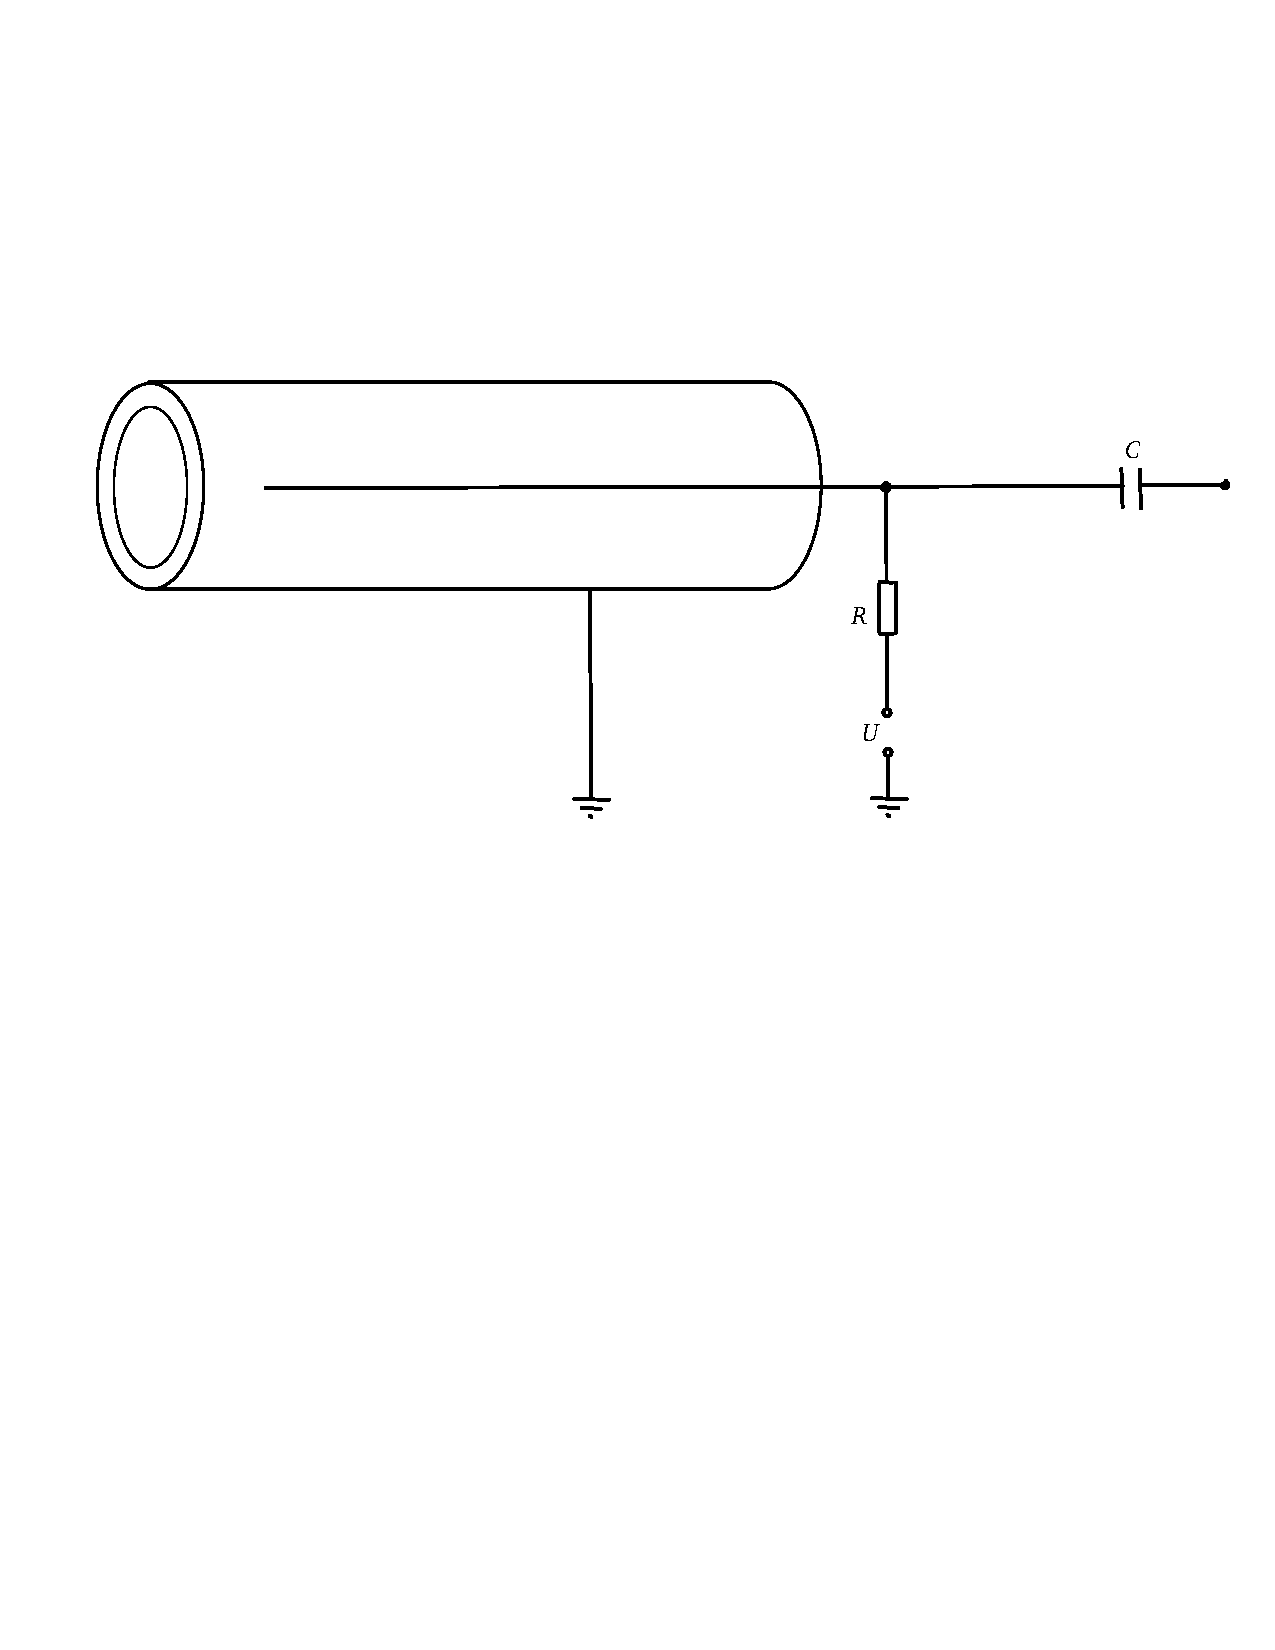
\includegraphics[width=\textwidth]{../Abbildungen/Geiger-Mueller.pdf}
    \caption{%
        Aufbau eines Geiger-Müller-Zählers
    }
    \label{fig:geiger}
\end{figure}

Der Aufbau eines Geiger-Müller-Zählrohres ist in Abbildung~\ref{fig:geiger} 
zu sehen. Sowohl die Spannung, als auch der Widerstand sind groß. Die 
Kammer mit dem etwa \SI{0.1}{\milli\meter} dicken Anodendraht ist mit einem 
Gasgemisch gefült, häufig werden Edelgase oder einfache Luft mit 
Ethanoldampf vermischt.

\FloatBarrier
\subsubsection{Funktionsweise}

Gelangt Strahlung in das Rohr werden vereinzelt Gasmoleküle ionisiert. Was
nun passiert kommt auf die angelegte Spannung an. Bei geringer Spannung
rekombinieren die Elektronen auf dem Weg zur Anode, was dafür sorgt, dass das
Signal keine brauchbaren Informationen liefert.

Bei einigen \SI{100}{\volt} lösen Elektronen nah der Anode durch Ionisation
weitere Ionen aus, es entstehen Elektronenlawinen mit bis zu \num{1e6}
Elektronen. Das entstehende Signal ist leicht messbar und proportional zur
durch die Strahlung im Zählrohr abgegebenen Energie. Daher wird das
Zählrohr in diesem Betrieb auch Proportionalzählrohr genannt.

Ab einer noch höheren Spannung erzeugt jede einfallende ionisierende
Strahlung Elektronenlawinen, die sich durch das ganze Rohr erstrecken. Das
entstehende Signal ist so groß, dass es ohne weitere Verstärkung zum
Beispiel in einem Lautsprecher ein Knacken erzeugen kann. In diesem Betrieb ist
das Zählrohr maximal empfindlich.

Ist die Spannung noch größer, braucht es keine einfallende Strahlung mehr um
das Gas zu Ionisieren, dies geschieht durch die Spannung allein. Das
Zählrohr ist in diesem Betrieb nicht mehr brauchbar.

\subsubsection{Totzeit}

Im Proportionalitäts- und Geiger-Müller-Betrieb des Zählrohrs schirmen die
entstehenden Ionen das Gas teilweise von der Spannung ab, was kurzzeitig
einen Betrieb verhindert. Erst wenn die Elektronen und Ionen rekombiniert
sind ist das Zählrohr wieder funktionsfähig. Die Zeit die es bis dahin
braucht nennt man Totzeit. Da im Geiger-Müller-Zähler das gesamte Gas
ionisiert ist, ist die Totzeit entsprechend groß, sie liegt in der
Größenordnung \SI{1e-4}{\second}.

Durch die Wahl des Gasgemischs kann die Rekombinations- und Totzeit
verringert werden.

\subsection{Röntgenenergiedetektor}

\subsubsection{Aufbau}

Kern eines Röntgenenergiedetektors ist die so genannte PIN-Photodiode.
Diese besteht aus einem Halbleiter, der zwischen einem $p$- und einem
$n$-dotierten Bereich einen undotierten (intrisischen) Bereich hat. Dieser
verhindert im normalbetrieb einen Stromfluss.

\subsubsection{Funktionsweise}

Trifft Röntgenstrahlung auf den intrinsischen Bereich, werden Elektronen
angeregt, und so ein freies Elektronen-Loch-Paar erzeugt. Da es zu dieser
Anregung nur wenige \si{\electronvolt} braucht, kann ein einfallender
Röntgenstrahl eine zu seiner Energie proportionale Anzahl an Paaren
erzeugen. Dadurch fließt in der Diode ein zur Röntgenenergie proportionaler
Strom, aus dem man die Energie ablesen kann.

\parencite[Abschnitt~„Photodiode“]{wikipedia/pin-Diode}

\subsubsection{Vielkanalanalysator}

Ein Vielkanalanalysator registriert die Spannungspulse, teilt diese in viele
Spannungsintervalle auf und zählt die Häufigkeit.
\parencite{Phywe/Vierkanalanalysator} So entsteht ein Histogram der Energien.
\parencite{wikipedia/Vielkanalanalysator}

\section{Röntgenfluoreszenz}

Wird ein Atom durch Röntgenstrahlung angeregt oder ionisiert, fallen
höherenergetische Elektronen in die frei gewordenen Löcher. Dabei strahlen
sie wie bei der Erzeugung charakteristischer Röntgenstrahlung isotrop
Energie in Form von erneuter Röntgenstrahlung ab, deren Spektrum für
verschiedene Atomkerne unterschiedlich ist. Dies bietet die Möglichkeit ein
Material zu untersuchen, ohne dieses zu zerstören.

\subsection{Bestimmung der Massenanteile}

Untersucht man eine Legierung mit Hilfe von Röntgenfluoreszens, erhält man
ein Spektrum, welches aus den überlagerten Spektren der einzelnen
Materialien besteht, nur mit unterschiedlich reduzierter Peakhöhe.

Um die tatsächlichen Anteile zu berechnen, kann man davon ausgehen, dass die
Peakhöhe $H$ proportional zur tatsächlichen Anzahl von Atomen $n$ ist.
Damit gilt:

\begin{align*}
    n &= n_0 \frac{H}{H_0}
    \intertext{Mit der Referenzanzahl}
    n_0 &= V \frac{\rho}{A} \intertext{%
        wobei $V$ das effektive Volumen, $\rho$ die Dichte und $A$ die
        Atommasse bezeichnen, erhält man
    }
    n &= V \frac{\rho}{A} \frac{H}{H_0}
    \intertext{%
        Den Massenanteil $C_i$ erhält man durch
    }
    C_i &= \frac{n_iA_i}{\sum_i n_iA_i} \\
        &= \frac{\rho_i\frac{H_i}{H_{0,i}}} {\sum_i\rho_i\frac{H_i}{H_{0,i}}}
\end{align*}


\parencite[„Massenanteilsbestimmung“]{physik412-Anleitung}

\FloatBarrier
\section{Bragg-Bedingung}

\begin{figure}
    \centering
    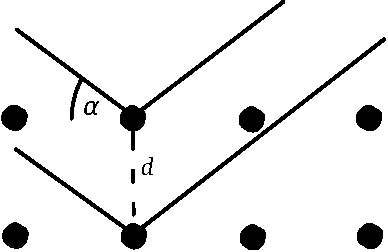
\includegraphics{../Abbildungen/Bragg.pdf}
    \caption{%
        Beugung im Kristallgitter
    }
    \label{fig:bragg}
\end{figure}

Trifft eine elektromagnetische Welle auf ein Kristallgitter, wird sie
an den Gitteratomen reflektiert. Dabei ändert sich die Wellenlänge nicht.
Die Situation ist in Abbildung~\ref{fig:bragg} skizziert.
Bei einem Winkel $\alpha$ zwischen einfallendem Strahl und Gitterebene ist
der Gangunterschied zwischen an benachbarten Gitterebenen reflektierten
Strahlen
\begin{align*}
    \Delta &= 2d\sin\alpha
    \intertext{%
        Damit konstruktive Interferenz stattfinden kann muss dieser
        Gangunterschied ein vielfaches der Wellenlänge sein:
    }
    n\lambda &= 2d\sin\alpha
\end{align*}
Dies ist die so genannte Bragg-Bedingung. Bei allen anderen Verhältnissen
zwischen Winkel, Wellenlänge und Netzebenenabstand, findet eine
vollständige Auslöschung statt.

\section{Laue-Bedingung}

Die Laue-Bedingung lautet
\[
    \Deltaup \vec k = \vec g
\]
das heißt, konstruktive Interferenz findet statt, wenn die Änderung des
Wellenvektors einem reziproken Gittervektor entsprechen. Im Grunde ist
diese Bedingung zur Bragg-Bedingung äquivalent, während Bragg jedoch von
quasi spiegelnden Ebenen ausgeht, formuliert von Laue seine Bedingung für
viele einzelne Streuzentren.

\parencite[(18.4)]{meschede-gerthsen_24}

\FloatBarrier
\section{Laue-Verfahren}

Beim Laue-Verfahren wird ein dünner Kristall mit weißer Röntgenstrahlung
bestrahlt. Hinter den Kristall wird im Abstand $L$ eine Photoplatte
gestellt. Die Bragg-Bedingung wird, da verschiedene Wellenlängen vorliegen,
vielfach erfüllt. Auf dem Schirm entsteht ein Punktmuster. Aus den
Koordinaten ($x$,$y$) der Punkte kann zunächst die dritte Koordinate mit
\[
    z = \sqrt{x^2 + y^2 + L^2} - L
\]
\parencite[P428.5.3, „Auswertung“]{physik412-Anleitung}

\subsection{Elementarzelle}

Die Elementarzelle einer Kristallstruktur, ist ein durch drei Vektoren
$\vec a_1$, $\vec a_2$ und $\vec a_3$ aufgespanntes Paralellepiped. Durch
periodische Wiederholung der Elementarzelle in alle Richtungen, wird das
ganze Kristallgitter aufgespannt.

\subsection{Millersche Indizes}

Um scharen paralleler Ebenen definieren zu können sind die Millerschen
Indizes hilfreich. Dabei legt man einen Punkt der Elementarzelle in den
Ursprung eines Koordinatensystems und betrachtet die Spurpunkte $s_1\vec
a_1$, $s_2\vec a_2$ und $s_3\vec a_3$ der Ebene. Nun bildet man die
Kehrwerte der $s_i$ und multipliziert mit einer ganzen Zahl, sodass die
Ergebnisse ebenfalls ganze Zahlen $h$, $k$, $l$ sind. Das Tupel $(hkl)$
heißt Millersche Indizes.

Liegt der Kristall beim Laue-Verfahren so, dass die Kristallachsen mit dem
Laborkoordinatensystem übereinstimmem, können die Millerschen Indizes der
reflektierenden Kristallebene über die Beziehung
\[
    h:k:l = x:y:z
\]
gefunden werden.

\subsection{Glanzwinkel}

Der Glanzwinkel kann aus einfachen geometrischen Überlegungen bestimmt
werden. Der einfallende Strahl hat einen Winkel von 0 zur optischen Achse. 
Da bei der Reflexion am Gitter Einfallswinkel und Ausfallswinkel gleich
groß sein müssen, ist der Austrittswinkel $2\theta$. Dieser kann mit Hilfe
der Punktkoordinaten berechnet werden:
\[
    \tan\del{2\theta} = \frac{\sqrt{x^2+y^2}}{L}
\]

\subsection{Netzebenenabstand}

In einem kubischen System mit Gitterkonstante $a_0$ kann man den
Netzebenabstand aus den Miller-Indizes mit
\[
    d = \frac {a_0} {\sqrt{ h^2 + k^2 + l^2}}
\]
berechnen. \parencite[Vorlesung~3]{physics613-Vorlesung}

\chapter{Bragg-Reflexion}

\section{Aufbau}

Wir benutzen ein Vollschutzröntgengerät, wobei wir eine unbekannte Anode
benutzen. \parencite{leybold/554800}

Für diesen Versuchsteil benutzen wir einen NaCl-Kristall
\footcite{wikipedia/hygroskopie} der Größe $\SI{25 +- 1}{\milli\meter}
\times \SI{25 +- 1}{\milli\meter} \times \SI{3.5 +- 0.5}{\milli\meter}$.

Kristall und Geigerzähler sind an einem elektrischen Goniometer angebracht, so
dass computergesteuert die Winkel durchfahren werden können.
\parencite{leybold/554831} \parencite{wikipedia/Goniometer}

Wir stellen den Taster am Gerät auf \textsc{coupled}, damit der Winkel des
Zählrohrs immer der doppelte Winkel der Probe ist. \parencite{leybold/554800}
Auf diese Weise erhalten wir eine optimale Bragg-Beugung und maximale
Intensität.

Dann setzen wir den groben Kollimator ein und stellen den Abstand zwischen
Kollimator und Kristallarm auf \SI{5}{\centi\meter} ein, den Abstand zwischen
Kristall- und Geigerzählerarm auf \SI{6}{\centi\meter}.

Zuletzt lassen wir die automatische Nullpunktbestimmung durch die Software
laufen.

\section{Bestimmung des Anodenmaterials}

\begin{figure}[htbp]
    \centering
    \includegraphics[width=\linewidth]{Roehre_2.pdf}
    \caption{%
        Spektrum der unbekannten Röhre mit Nummer 2.
    }
    \label{fig:}
\end{figure}

\subsection{Auswertung}

Wir benutzen eine Gitterkonstante von $d = \SI{<< nacl_a >>}{\meter}$.
\parencite{Unkelbach/Bragg_Zusatzaufgaben}. Dies ist die Hälfte der Konstante,
die auf \cite{wikipedia/Natriumchlorid} angegeben ist.

Dabei gehen wir davon aus, dass dies die Linien das Paar $K_\beta$ und
$K_\alpha$ in mehreren Ordnungen sind. Die Maxima sind an Vielfachen der ersten
Position, außerdem kann man bei \SI{24}{\degree} noch ein kleines Maximum
erkennen, dies wird die vierte Ordnung sein.

Die Wellenlängen erhalten mit den entsprechenden $n$ wie folgt:
\[
    \lambda = 2 \frac dn \sin(\beta).
\]

Die Maxima haben folgende Wellenlängen: \SIlist{<< r2_lambda_pm
>>}{\pico\meter}.

Die entsprechenden Energien erhalten wir mit
\[
    E = \frac{c h}{\lambda}.
\]

In $\si{\kilo\electronvolt}$ umgewandelt ist die Liste dann: \SIlist{<<
r2_e_kev >>}{\kilo\electronvolt}.

Laut \cite[Tabelle~1-2]{x-ray_data_booklet}, entsprechen die $K_\alpha$- und
$K_\beta$-Linien derer von Indium. Somit gehen wir davon aus, dass das
Anodenmaterial von Röhre~2 Indium ist.

\section{Feinstrukturmessung}

Unsere Messdaten sind in Abbildung~\ref{fig:Langzeit} dargestellt.

\begin{figure}[htbp]
    \centering
    \includegraphics[width=\linewidth]{Langzeit.pdf}
    \caption{%
        Spektrum der Molybdän-Röhre. Es ist die Aufspaltung der
        $K_\alpha$-Linie in vierter Beugungsordnung zu sehen.
    }
    \label{fig:Langzeit}
\end{figure}

\subsection{Auswertung}

Da wir in vierter Ordnung gemessen haben, ist die Formel jetzt
\[
    \lambda = \frac24 d \sin(\beta).
\]

Wir rechnen entsprechend die Wellenlängen in Energien um.

Unsere gemessenen Peaks entsprechen Energien von \SIlist{<< langzeit_e
>>}{\kilo\electronvolt}. Bei Molybdän sind die Energien \SIlist{<<
langzeit_e_mo >>}{\kilo\electronvolt} zu erwarten.
\parencite[Tabelle~1-2]{x-ray_data_booklet} Dies passt recht gut.

Die Energieaufspaltung der $K_\alpha$ Linie ist bei den Literaturwerten \SI{<<
aufspaltung_literatur >>}{\percent}, bei unserer Messung ist es \SI{<<
aufspaltung_gemessen >>}{\percent}. Die beiden Werte passen gut zusammen.

\chapter{Zerstörungsfreie Aufnahme chemischer Zusammensetzungen}

In diesem Versuchsteil untersuchen wir eine Metalllegierung und versuchen ihre
Bestandteile herauszufinden.

\section{Aufbau}

Wir benutzen die Kupferanode und stellen das Goniometer so ein, dass die Probe
auf \SI{45}{\degree} liegt und der Energiedetektor auf \SI{90}{\degree} steht.

Am Computer stellen wir die Vielkanalmessung mit 512 Kanälen ein. Negative
Pulse. Wir setzen die Verstärkung auf \num{-2.5} und die Messdauer auf
\SI{180}{\second}.

\section{Kalibrierung mit FeZn}

Zuerst müssen wir die Energie kalibrieren. Dies bedeutet, dass wir einem
Energiekanal eine Energie in \si{\electronvolt} zuordnen können.

\subsection{Durchführung}

Wir legen das Plättchen mit FeZn auf den Probenhalter und nehmen ein Spektrum
auf. Dies ist in Abbildung~\ref{fig:FeZn} gezeigt.

\begin{figure}[htbp]
    \centering
    \includegraphics[width=\linewidth]{FeZn.pdf}
    \caption{%
        Spektrum von FeZn.
    }
    \label{fig:FeZn}
\end{figure}

\subsection{Auswertung}

Nun schauen wir \cite[Tabelle~1-2]{x-ray_data_booklet} nach den Energien für
die $K_\alpha$ Linie von Eisen und Zink nach. Mit diesen beiden Datenpunkten
können wir die Energieanpassung vornehmen und mit einer linearen Funktion
anpassen. Diese Funktion ist in Abbildung~\ref{fig:Energieeichung} dargestellt.

\begin{figure}[htbp]
    \centering
    \includegraphics[width=\linewidth]{Energieeichung.pdf}
    \caption{%
        Anpassung der Energie an die Kanalnummer.
    }
    \label{fig:Energieeichung}
\end{figure}

Als Transformation von Kanal $K$ zur Energie $E$ erhalten wir:
\[
    E(K) = a K + b
    \eqnsep
    a = \SI{<< energie_steigung >>}{\electronvolt}
    \eqnsep
    b = \SI{<< energie_abschnitt >>}{\electronvolt}
\]

Jetzt können wir in den weiteren Spektren anstelle der Kanalnummer eine Energie
schreiben.

\section{Aufnahme der Legierung}

\subsection{Durchführung}

Wir tauschen das FeZn-Plättchen gegen die Probe~1 und nehmen erneut das
Spektrum auf. Das Spektrum ist in Abbildung~\ref{fig:Probe_1} gezeigt.

\begin{figure}[htbp]
    \centering
    %\includegraphics[width=\linewidth]{Probe_1.pdf}
    \caption{%
        Spektrum der unbekannten Probe~1.
    }
    \label{fig:Probe_1}
\end{figure}

\section{Aufnahme der reinen Metalle}

Nun gehen wir nacheinander alle Metalle durch, die wir zur Verfügung haben und
nehmen je ein Spektrum auf.

\section{Bestimmung der Legierung und Massenanteile}

Wir tragen alle normalisierten Spektren der Metalle zusammen in einem Diagramm
ein, siehe Abbildung~\ref{fig:Bestimmung}. Da wir daran interessiert sind, die
Maxima der Probe~1 zu erklären, wählen wir einen entsprechenden Ausschnitt.

\begin{figure}[htbp]
    \centering
    \includegraphics[width=\linewidth]{Bestimmung.pdf}
    \caption{%
        Spektra der unbekannten Probe sowie der reinen Metalle. Die Spektra
        sind normalisiert, so dass die Amplitude des Hauptmaximums gerade 1
        ist. 
    }
    \label{fig:Bestimmung}
\end{figure}

Es ist zu erkennen, dass das Hauptmaximum durch Eisen erzeugt wird. Das kleine
Maximum ist allerdings durch kein anderes Spektrum zu erklären. In der
Vergrößerung in Abbildung~\ref{fig:Bestimmung_Zoom} wird dies noch deutlicher.

\begin{figure}[htbp]
    \centering
    \includegraphics[width=\linewidth]{Bestimmung_Zoom.pdf}
    \caption{%
        Ausschnittsvergrößerung von Abbildung~\ref{fig:Bestimmung}
    }
    \label{fig:Bestimmung_Zoom}
\end{figure}

Daher haben wir in \cite{x-ray_data_booklet} nachgeschlagen und gefunden, dass
das Element Chrom dort eine helle Linie hat. In dieser Legierung scheint also
Eisen und Chrom zu sein.

Die maximale Amplitude bei Eisen ist \num{<< fe_max >>}, in der
Eisen-Chrom-Probe ist es \num{<< fecr_max >>}. Aus dem Verhältnis können wir
schließen, dass der Atomanteil von Eisen $n_\text{Fe} = \SI{<< fecr_fe_prozent
>>}{\percent}$ beträgt. Wir nehmen an, dass die verbleibenden $n_\text{Cr} =
\SI{<< cr_prozent >>}{\percent}$ der Atome Chrom sind. Mit Atomgewichten von
$A_\text{Fe} = \SI{<< A_fe >>}{\atomicmassunit}$\footcite{wikipedia/Eisen} und
$A_\text{Cr} = \SI{<< A_cr >>}{\atomicmassunit}$\footcite{wikipedia/Chrom} für
Eisen bzw. Chrom können wir nun die Formel aus der Anleitung für die
Massenanteile ausnutzen
\[
    C_i = \frac{n_i A_i}{\sum_j n_j A_j}
    \eqnsep
    i, j \in \set{\text{Fe}, \text{Cr}}
\]
und erhalten:
\[
    C_\text{Fe} = \SI{<< C_fe >>}{\percent}
    \eqnsep
    C_\text{Cr} = \SI{<< C_cr >>}{\percent}.
\]

\chapter{Laue-Aufnahme}

In diesem Versuchsteil untersuchen wir das Beugungsmuster an einem NaCl
Kristall.

\section{Aufbau}

Wir benutzen die Röntgenröhre mit der Kupferanode mit einer Hochspannung von
\SI{35}{\kilo\volt} und einem Emissionsstrom von \SI{1}{\milli\ampere}.

Auf den groben Kollimator wird der NaCl Kristall aufgesteckt. Der Film (AGFA
Dentus M2 Comfort Röntgenfilm) wird mit dem entsprechenden Halter im Querformat
in einem Abstand von \SI{15}{\milli\meter} zum Kristall angebracht.

\section{Durchführung}

Die Strahlung wird für \SI{1800}{\second} betrieben. Danach entnehmen wir den
Film und entwickeln ihn gemäß ausliegender Anleitung mit Entwickler und
Fixierer.

Nachdem wir den Film fertig entwickelt haben, haben wir ihn getrocknet und mit
600 DPI eingescannt. Das Bild ist in Abbildung~\ref{fig:laue} gezeigt.

\begin{figure}[htbp]
    \centering
    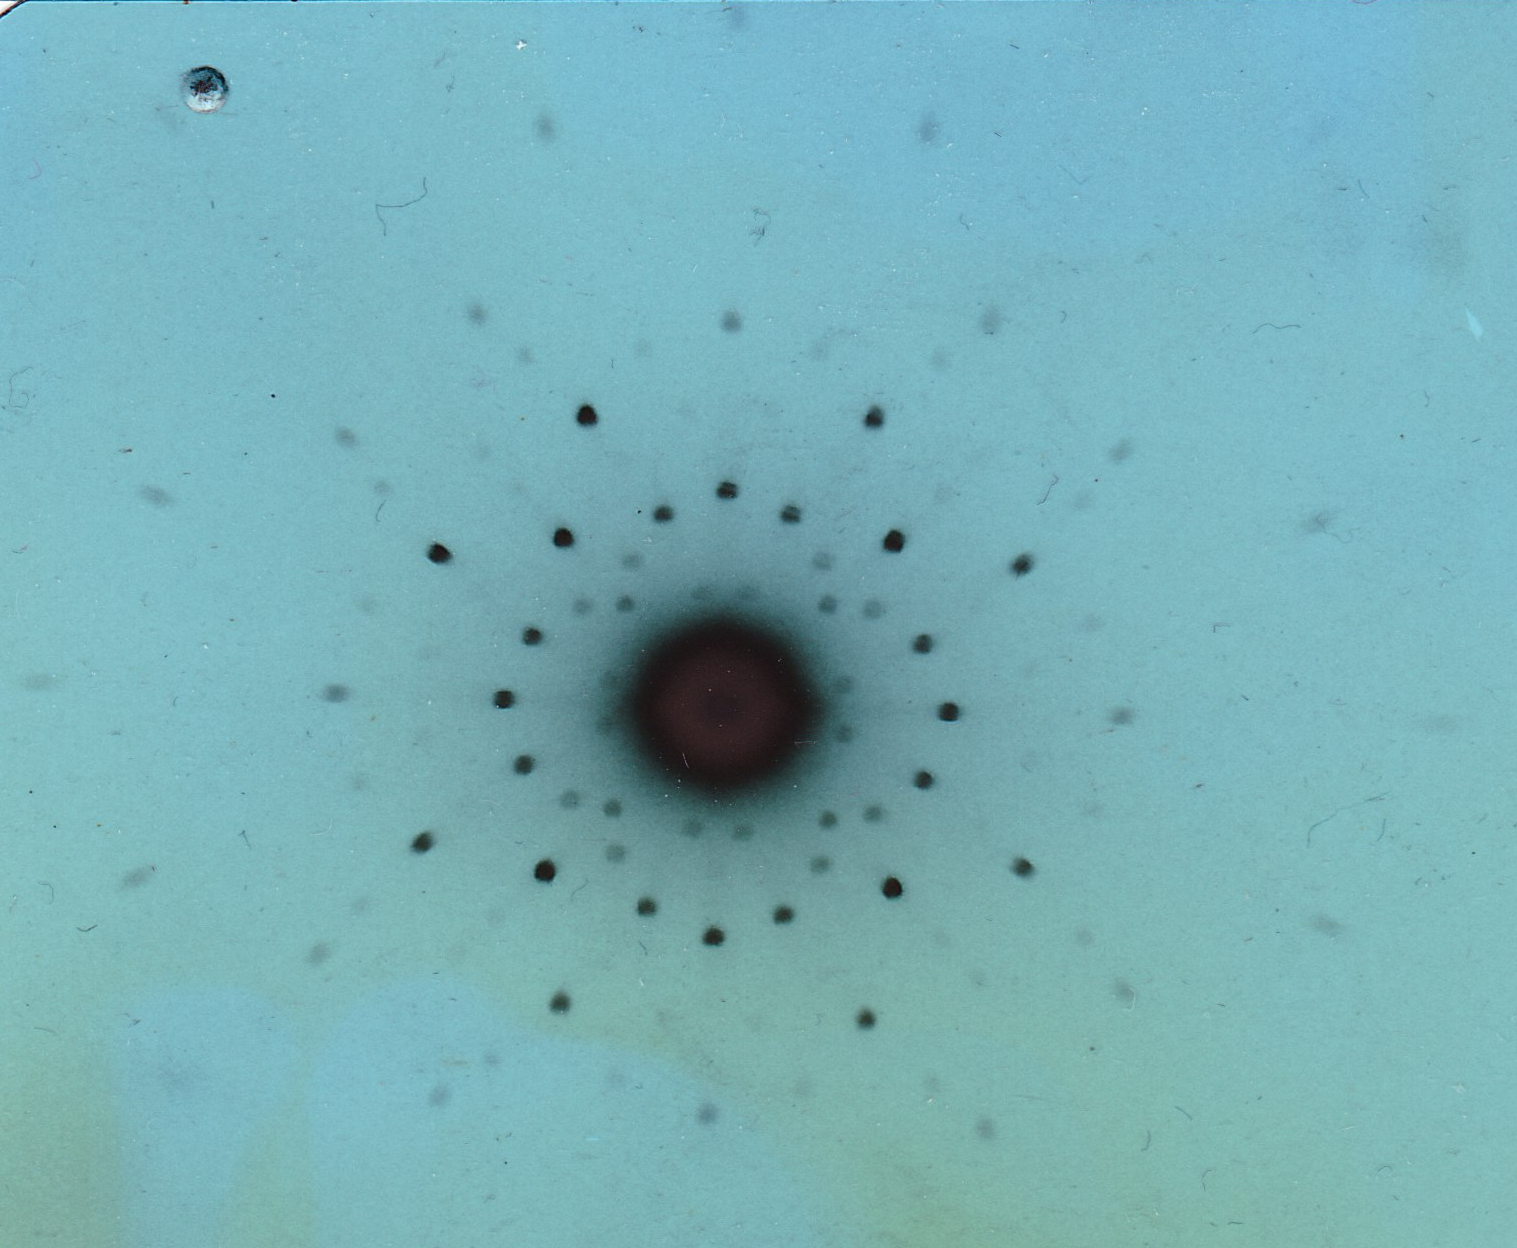
\includegraphics[width=\linewidth]{../Messdaten/laue.png}
    \caption{%
        Scan des Fotos, das wir durch Beugung an einem NaCl-Kristall erzeugt
        haben. 600 DPI.
    }
    \label{fig:laue}
\end{figure}

\section{Auswertung}

Um das Bild analysieren zu können, haben wir aus den RGB-Daten den blauen Kanal
herausgenommen. Wir hätten auch Mittelwerte, Maxima oder ähnliches nehmen
können. Jedoch ist das ganze Bild etwas bläulich, so dass uns dies gut
erschien. Der Helligkeitswert ist in Abbildung~\ref{fig:laue-helligkeit}
dargestellt. Die Abbildung ist jedoch in Falschfarben, um die Helligkeit besser
sichtbar zu machen.

\begin{figure}[htbp]
    \centering
    \includegraphics[width=\linewidth]{laue-helligkeit.pdf}
    \caption{%
        Helligkeit im blauen Kanal.
    }
    \label{fig:laue-helligkeit}
\end{figure}

Gegen das unvermeidliche Rauschen durch den Scanner und den Film haben wir das
Bild geglättet. Dazu haben wir eine Gauß'sche
Unschärfe\footnote{\texttt{scipy.ndimage.filters.gaussian\_filter}} benutzt, die
nacheinander eine Faltung in  $x$ und $y$ mit einem Gaußkern vornimmt. Dabei
haben wir als Radius << gauss_radius >> Pixel benutzt. Das geglättete Bild ist
in Abbildung~\ref{fig:laue-gauss}.

\begin{figure}[htbp]
    \centering
    \includegraphics[width=\linewidth]{laue-helligkeit-gauss.pdf}
    \caption{%
        Helligkeit nach Gauß'scher Unschärfe mit << gauss_radius >> Pixeln
        Radius.
    }
    \label{fig:laue-gauss}
\end{figure}

An der Skala am rechten Rand von Abbildung~\ref{fig:laue-gauss} ist zu
erkennen, dass der Wertebereich der Helligkeit kleiner geworden ist. Die ganz
dunklen und hellen Stellen wurden geschwächt. Der Kontrast hat also abgenommen,
jedoch werden die nächsten Schritte dadurch zuverlässiger.

\subsection{Ablesen der Reflexpunkte}

Um die Punkte algorithmisch finden zu können, wollen wir den Laplaceoperator
auf die Helligkeit anwenden. Dazu bilden wir zuerst den
Gradient\footnote{\texttt{numpy.gradient}}. Das Zwischenergebnis ist in
Abbildung~\ref{fig:laue-gradient} gezeigt.

\begin{figure}[htbp]
    \centering
    \includegraphics[width=\linewidth]{laue-gradient_x_y.pdf}
    \caption{%
        Amplitude des Gradients der Helligkeit.
    }
    \label{fig:laue-gradient}
\end{figure}

Dann bilden wir die Divergenz des Gradienten und erhalten die Quellendichte.
Siehe Abbildung~\ref{fig:laue-laplace}.

\begin{figure}[htbp]
    \centering
    \includegraphics[width=\linewidth]{laue-laplace}
    \caption{%
        Quellendichte der Helligkeit. Diese wurde mit dem Laplaceoperator
        bestimmt.
    }
    \label{fig:laue-laplace}
\end{figure}

Jetzt sind die Reflexionen besser vom Hintergrund abgehoben. Mit den Daten aus
Abbildung~\ref{fig:laue-helligkeit} oder \ref{fig:laue-gauss} wäre es nicht
möglich gewesen durch eine untere Grenze so viele Reflexionen zu isolieren.

Wir wenden nun eine untere Grenze von \num{<< laplace_threshold >>} an, um die
Maxima zu isolieren. Dann lassen wir die verbleibenden Objekte im Bild
suchen.\footnote{\texttt{scipy.ndimage.label} und
\texttt{scipy.ndimage.find\_objects}}

Zur Kontrolle sind in Abbildung~\ref{fig:laue-peaks} die gefundenen Reflexionen
eingezeichnet.

\begin{figure}[htbp]
    \centering
    \includegraphics[width=\linewidth]{laue-peaks.pdf}
    \caption{%
        Gefundene Maxima über einem Schwellenwert von \num{<< laplace_threshold
        >>}.
    }
    \label{fig:laue-peaks}
\end{figure}

\subsection{Zuordnung der Gitterebenen}

Die Koordinaten korrigeren wir noch so, dass die Mitte gerade bei 0 liegt. Dazu
ziehen wir von $x$ \num{<< x_offset >>} und von $y$ \num{<< y_offset >>} ab. Da
das Bild mit 600 DPI eingescannt worden ist, können wir $x$ und $y$ von Pixeln
in Meter umwandeln. Zusammen mit $L = \SI{15}{\milli\meter}$ können wir dann
$z$ berechnen:
\[
    z = \sqrt{x^2 + y^2 + L^2} - L
\]

Wir bilden die beiden Verhältnisse
\[
    A := \frac xz
    \eqnsep
    B := \frac yz
\]
und lassen diese als Brüche mit kleinem Nenner
darstellen\footnote{\texttt{fractions.Fraction} mit
\texttt{fractions.Fractions.set\_denominator}}. Aus dieser Darstellung
errechnen wir die drei Laue-Indizes wie folgt:
\begin{align*}
    h &= \frac{A_\text{Zähler}}{A_\text{Nenner}}
    \mathop{\mathrm{kgv}}(A_\text{Nenner}, B_\text{Nenner}) \\
    k &= \frac{B_\text{Zähler}}{B_\text{Nenner}}
    \mathop{\mathrm{kgv}}(A_\text{Nenner}, B_\text{Nenner}) \\
    l &= \mathop{\mathrm{kgv}}(A_\text{Nenner}, B_\text{Nenner})
\end{align*}

Die so errechneten Laue-Indizes sind an die Stellen des Reflexes in
Abbildung~\ref{fig:laue-indizes} eingetragen. Dabei bedeutet die
Überstreichung, dass der entsprechende Werte negativ ist.

\begin{figure}[htbp]
    \centering
    \includegraphics[width=\linewidth]{laue-indizes.pdf}
    \caption{%
        Errechne Laue-Indizes zu den Reflexionen.
    }
    \label{fig:laue-indizes}
\end{figure}

Alle in Abbildung~\ref{fig:laue-indies} Gitterebenen haben wir in
Tabelle~\ref{tab:laue-index}

\begin{table}[htbp]
    \centering
    \begin{tabular}{SSSS|cSSS}
        {$x / \si{\milli\meter}$} & {$y / \si{\milli\meter}$} & {$A$} & {$B$} & Ebene & {$\theta / \si\degree$} & {$d / \si{\pico\meter}$} & {$\lambda /
    \si{\pico\meter}$} \\
        \midrule
        %< for a, b, c, d, e, f, g, h in laue_tabelle: ->%
        << a >> & << b >> & << c >> & << d >> & << e >> & << f >> & << g >> &
        << h >> \\
        %< endfor ->%
    \end{tabular}
    \caption{%
        Errechnete Glanzwinkel $\theta$ und Ebenenabstände $d$. Die Daten sind
        nach absteigendem Glanzwinkel sortiert.
    }
    \label{tab:laue-index}
\end{table}

Bei der Zurodnung

\chapter{Zusammenfassung}

\chapter{Diskussion}

%%%%%%%%%%%%%%%%%%%%%%%%%%%%%%%%%%%%%%%%%%%%%%%%%%%%%%%%%%%%%%%%%%%%%%%%%%%%%%%
%                                   Anhang                                    %
%%%%%%%%%%%%%%%%%%%%%%%%%%%%%%%%%%%%%%%%%%%%%%%%%%%%%%%%%%%%%%%%%%%%%%%%%%%%%%%

\FloatBarrier
\begin{appendix}
    \FloatBarrier
    \chapter{\LaTeX-Quelltext}

    Der \LaTeX-Quelltext zu allen Protokollen in diesem Praktikum kann auf
    \ref{it:mu} eingesehen werden. Die Quellen für alle Protokolle in diesem
    Praktikum können auf \ref{it:github/alles} eingesehen werden. Die
    \LaTeX-Datei wird aus \ref{it:github/template} generiert.

    \begin{enumerate}
        \item
            \label{it:mu}
            \url{http://martin-ueding.de/de/university/physik412/}
        \item
            \label{it:github/alles}
            \url{https://github.com/martin-ueding/physik412-Protokolle/}
        \item
            \label{it:github/template}
            \url{https://github.com/martin-ueding/physik412-Protokolle/blob/master/\versuchsnummer/Template.tex}
    \end{enumerate}
\end{appendix}

%%%%%%%%%%%%%%%%%%%%%%%%%%%%%%%%%%%%%%%%%%%%%%%%%%%%%%%%%%%%%%%%%%%%%%%%%%%%%%%
%                                  Literatur                                  %
%%%%%%%%%%%%%%%%%%%%%%%%%%%%%%%%%%%%%%%%%%%%%%%%%%%%%%%%%%%%%%%%%%%%%%%%%%%%%%%

\FloatBarrier
\printbibliography

\end{document}

% vim: et spell spelllang=de tw=79
